% Compile with TeX Live: xelatex -interaction=nonstopmode -halt-on-error 刘元智_简历.tex
\documentclass[UTF8,fontset=fandol,a4paper]{ctexart}
\usepackage[left=8mm,right=8mm,top=8mm,bottom=8mm]{geometry}
\usepackage{fontspec,graphicx,xcolor,enumitem,tikz,eso-pic,hyperref}
\setmainfont{Times New Roman}
\hypersetup{hidelinks,pdfauthor={刘元智},pdftitle={刘元智简历}}
\pagestyle{empty}
\linespread{1}
\setlength{\parindent}{0pt}
\setlength{\parskip}{2pt}
\setlist[itemize]{leftmargin=15pt,labelsep=5pt,topsep=1pt,itemsep=2pt,parsep=0pt,partopsep=0pt}
\definecolor{resumeBlue}{HTML}{4080FF}
\definecolor{resumePale}{HTML}{B2CCFF}
\AddToShipoutPictureBG{%
  \AtPageUpperLeft{\raisebox{-80mm}{
\includegraphics[width=\paperwidth,height=80mm]{assets/X4.png}}}}
\newcommand{\sectionline}[1]{%
  \par\addvspace{9pt}
  \noindent
\begin{tikzpicture}[baseline=-2pt]
    \fill[resumePale] (2.5pt,0) -- (11pt,6pt) -- (2.5pt,12pt) -- cycle;
    \fill[resumeBlue] (0,0) -- (8.5pt,6pt) -- (0,12pt) -- cycle;
  \end{tikzpicture}\hspace{5pt}%
  {\color{resumeBlue}\bfseries\fontsize{12}{15}\selectfont #1}%
  \hspace{7pt}{\color{resumeBlue}\leaders\hrule height .55pt\hfill}\kern0pt
  \par\nobreak\vspace{3pt}}
\newcommand{\entry}[2]{\par\noindent\textbf{#1}\hfill #2\par\nobreak}
\newcommand{\internship}[3]{%
  \par\addvspace{9pt}\noindent\textbf{#1}\hfill
  \raisebox{-3pt}[12pt][3pt]{\includegraphics[width=15pt,height=15pt,keepaspectratio]{#2}}%
  \hspace{9pt}#3\par\nobreak}
\newcommand{\tag}[1]{{\color{resumeBlue}\setlength{\fboxsep}{2pt}\colorbox{resumePale!25}{#1}}}
\begin{document}
\fontsize{9.5}{12.1}\selectfont

\noindent
\begin{minipage}[t]{24mm}
  \vspace{0pt}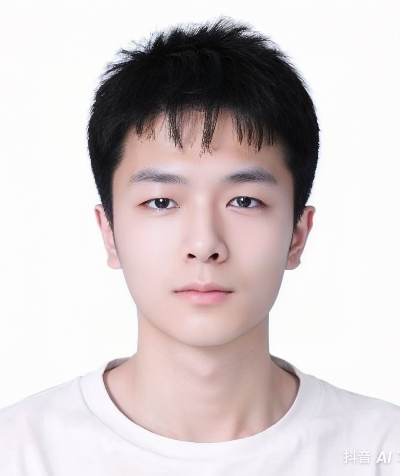
\includegraphics[width=21mm]{assets/X84.png}
\end{minipage}\hspace{3mm}%
\begin{minipage}[t]{105mm}
  \vspace{3mm}
  {\fontsize{17}{22}\selectfont\bfseries 刘元智}\par
  \vspace{5pt}
  电话：15769057937 | 邮箱：1739727979@qq.com\par
  年龄：24岁 | 性别：男 | 政治面貌：共青团员
\end{minipage}\hfill
\begin{minipage}[t]{49mm}
  \vspace{0pt}
\includegraphics[width=49mm]{assets/X85.png}
\end{minipage}
\vspace{5pt}

\sectionline{教育经历}
\entry{中国石油大学(北京)\quad \tag{211}\ \tag{双一流}}{2024年09月 - 2027年06月}
计算机技术 硕士 全日制\par
\entry{中国石油大学(北京)\quad \tag{211}\ \tag{双一流}}{2020年09月 - 2024年06月}
软件工程 本科 全日制

\sectionline{实习经历}
\internship{Shopee（北京）}{assets/shopee.png}{2025年09月 - 至今}
\textbf{岗位描述：}负责机器学习平台后端研发工作；负责流量调度服务后端研发工作；负责LLM-Gateway后端开发工作；\par
\textbf{工作内容：}
\begin{itemize}
  \item \textbf{需求开发：}负责AIS平台\textbf{v1.18～v1.21}的需求开发。MLP内部业务通过\textbf{Istio}进行流量转发，基于原生能力进行服务端适配，平台控制面提供限流重试、状态重置等相关配置并落库同步至服务Pod；
  \item \textbf{插件开发：}推理流量通过\textbf{RPC服务}进行调度；将部分计算任务迁移为沙箱，在QPS 2k的情况下将请求的\textbf{P99 RT降低约5\%}；
  \item \textbf{流量调度：}参与流量调度服务算法的若干实现，包括轮询、随机、前缀缓存等路由算法，使得平均推理 \textbf{TTFT 降低约13\%}；
  \item \textbf{模型评估：}Maas产品化涉及\textbf{大模型压测}，需要在满足业务延迟条件下评估推理服务所能支持的\textbf{最大TPS}；在工程侧负责压测阶段的相关链路，同步至集群侧；支持自定义配置，以获取大模型\textbf{TU、TUPM}折算系数进行内部定价；
  \item \textbf{推理网关：}负责内部统一推理网关开发，\textbf{接入5+供应商，30+相关模型}，涵盖OpenAi、Anthropic等若干家供应商；涉及文本、视频、多模态、JEV等若干类型大模型，提供推理能力；
  \item \textbf{自动治理：}AIS内部推理服务需要研发手动治理告警；基于\textbf{OpenClaw}搭建治理Bot，扩展Skill及工具Tool，根据运维文档标准自动化治理实例，\textbf{支持扩容、重启}等相关运维操作，日均处理\textbf{20+}服务告警；
\end{itemize}

\internship{字节跳动（北京）}{assets/bytedance.png}{2025年03月 - 2025年07月}
\textbf{岗位描述：}负责地理位置中台离线任务数据监控治理、内部AI专项提效；负责后端相关需求开发工作；\par
\textbf{工作内容：}
\begin{itemize}
  \item \textbf{质量保障：}基于Bamboo平台，监控内部若干团队3k+ Hive表生产数据，检测维度包括异常表行数、数据异常波动率等；设计\textbf{DVAD算法}以适配波动率抖动情况。存量监控通过平台定时触发检测任务，增量表通过接口形式同步至平台侧；
  \item \textbf{告警治理：}质量保障的需求延伸。设计并搭建\textbf{告警推送链路}。统计群内未响应告警，设定Aily Agent及相关工具提取信息，对接飞书API，由WorkFlow主动触及相关RD，将告警ACK率从\textbf{40\%}提升至\textbf{73\%}；
  \item \textbf{反馈打标：}负责不同Oncall工单打标。设计并搭建RAG方式的打标链路，基于字节内部开放模型获取推理能力，并搭建存量Oncall工单知识库，在该链路上将工单的打标准确率从\textbf{50\%提升至90\%}；
  \item \textbf{MCP工具：}AIDP业务团队问答BOT需要扩展工具能力，负责设定相关参数及DB筛选条件，搭建内部数据库读写接口。
\end{itemize}

\internship{爱诗科技（北京）}{assets/aisphere.png}{2024年11月 - 2025年02月}
\textbf{岗位描述：}负责大规模分布式系统研发工作，优化系统性能；负责海量数据的获取、清洗、交付工作；\par
\textbf{工作内容：}
\begin{itemize}
  \item \textbf{数据量：}内存使用量存在峰值抖动情况，定位原因为切片合并上传代码段。采取\textbf{子进程流式读取并落盘}，主进程\textbf{聚合元信息}，并调控多进程的\textbf{分配数量}，以解决32GB内存下数据处理的OOM问题；
  \item \textbf{流水线：}数据处理涉及多个流程，该功能点从DB角度映射Job、Task的Pre和Next状态，在上一个Job和对应Task完成后自动创建下一个\textbf{Jon的元信息}，以进行数据处理。目前支持\textbf{Job和Task级别}的流水线处理。
  \item \textbf{公平调度：}Master多实例调度Task状态，使用Redis分布式锁\textbf{隔离调度请求}，存在Corner情况\textbf{单实例多次调度}，通过\textbf{Redis List}和\textbf{Master UUID}，实现Redis的\textbf{轮转公平锁}以调度任务状态，确保多实例调度的顺序公平性。
  \item \textbf{心跳机制：}Worker节点不稳定，该机制通过记录\textbf{Task心跳}，由Worker节点定时更新，Master监控，进行切片重置；
\end{itemize}

\sectionline{项目经历}
\entry{Compass-Gateway}{2026年06月 - 至今}
\begin{itemize}
  \item \textbf{核心技术：}Golang、Python、Gin、Trace、MySQL、Redis、Kafka、Prometheus、Pipeline
  \item \textbf{项目描述：}Shopee内部大模型统一网关，提供MLP AIS平台推理服务及外部供应商模型服务。为Shopee内部用户提供模型推理能力。平台整体承载约 150+API 路由、20+模型供应商、200+模型。系统QPS 2000+。
\end{itemize}

\newpage
主要功能点：
\begin{itemize}
  \item \textbf{权限分配：}系统以\textbf{BU、Team、Project}维度进行权限拆分和分配，用户可根据自身权限自定义管理相关团队成员，并支持由PM进行Shopee、Garena、Migoo子公司级别的团队管控以及相关额度、模型可见性等若干配置。
  \item \textbf{预算配额：}团队预算方案存在差异，系统涵盖\textbf{CQP、AQP、DQP}等预算方案，其开放额度与内部IT Center\textbf{工单适配}，用户自定义提交工单以申请额度，系统根据工单状态做内部DB适配，以API-KEY形式对接用户额度，并进行相关额度的配置。
  \item \textbf{模型推理：}目前系统提供\textbf{内部MLP模型推理服务和外部供应商模型服务}，内部MLP平台推理模型服务根据单次推理的TU、TPM进行计费处理，外部供应商模型采用相关API的Token计价方式进行统一收费。
  \item \textbf{日志审计：}审计方式依赖HIve表，系统将单次推理请求通过Kafka同步至Hive表，配置\textbf{监控大盘}以并通过相关SQL聚合相关审计信息，以方便用户审查团队额度使用情况。在团队额度超出限额时自动发送相关通知信息。
\end{itemize}

\vspace{9pt}
\entry{TidalStation}{2024年11月 - 2025年02月}
\begin{itemize}
  \item \textbf{核心技术：}MongoDB、Redis、Kubernetes、Docker、Thrift、MLP、VEPFS
  \item \textbf{项目描述：}分布式数据处理平台，旨在利用业务中的潮汐资源完成数据处理的业务支持。
\end{itemize}
主要功能点：
\begin{itemize}
  \item \textbf{并行处理：}将数据集拆分为若干\textbf{切片}保存至MongoDB及Tos，对应若干Task，通过MLP平台启动若干实例并行处理数据；
  \item \textbf{任务调度：}Worker在获取任务后将信息同步至Master，由k8s负载将\textbf{流量分发}至Master实例监控任务运行状态，\textbf{轮询检测}Task状态并进行任务状态的调度，当前系统支持\textbf{3.8w/s}的轮询请求；
  \item \textbf{任务容错：}在启动闲时资源的情况下，单个Task存在因\textbf{资源调度}而失败的情况，系统支持在\textbf{非UDF失败}的情况下进行任务的\textbf{自动重试}，以适应火山资源动态分配的情况，在获得闲时资源后重新执行任务；
  \item \textbf{Pipeline：}数据集的处理涉及若干流程，该功能将多个数据处理流程合并为一条Pipeline，每条Pipeline将自动化处理流水线上的数据，并支持\textbf{批处理模式}及\textbf{伪流处理模式}，提升CPU及GPU的利用率；
\end{itemize}

\sectionline{研究经历}
\entry{量子扩散模型渗透率场生成及其预测研究}{2025年06月 - 2027年06月}
\begin{itemize}
  \item 量子注意力扩散模型（\href{https://github.com/Anyoneself/quantum-attention-net}{https://github.com/Anyoneself/quantum-attention-net}）
\end{itemize}
\hspace*{15pt}面向二维非均质渗透率场重构，设计融合空间自注意力与参数化量子门控的 U-Net 扩散模型；在存档的原型辅助评估中取得 RMSE 0.01225，较 GAN 基线的 0.05466 降低 77.6\%，并通过无网络对照分析原型注入对结果的影响。
\begin{itemize}
  \item 量子PINN网路模型（\href{https://github.com/Anyoneself/quantum-pinn-net}{https://github.com/Anyoneself/quantum-pinn-net}）
\end{itemize}
\hspace*{15pt}面向稀疏观测下的渗透率场补全，设计量子启发的可学习周期相位编码与门控坐标网络；在 128 幅数值场、相同训练轮数下，原始预测 RMSE 较固定 FNN 网络基线降低 9\%，并完成消融、抗噪及 Darcy 流动响应评估。

\sectionline{荣誉奖项}
挑战杯人工智能+赛道国奖、蓝桥杯大赛省奖、全国大学生数学建模竞赛省奖、科技创新先进个人奖学金、校级奖学金若干

\sectionline{技术栈}
\begin{itemize}
  \item 语言：熟悉Go、Java、Python语法，熟悉常用数据结构及其相关使用；
  \item 数据库：熟悉MySQL，MongoDB；熟悉Redis相关业务场景；
  \item 框架：熟悉Web开发主流框架，如Spring全家桶、Gorm、Heartz等；
  \item 大模型：熟悉Transformer架构、Langchain、RAG、Agent等大模型相关技术；
  \item 工具：熟练掌握Git、Docker、kubernetes等开发工具；
\end{itemize}

\sectionline{其他}
\begin{itemize}
  \item \textbf{语言：}英语（CET-6）
\end{itemize}
\end{document}
